\section{Design Models}
These models represent the concrete class diagrams which are planned and are to
be implemented

\subsection{Behavioral Modules}

\subsubsection{Diabetes}

\subsubsection{Food}
In order to provide the possibility for extensive and intuitive testing for the
food module also some GUI components have been designed.
These components include a frontend for input (e.g. adding food to the
simulation etc.) and a display of the output.

In order to provide large flexibility with respect to future changes the
concrete food types inherit from an abstract class. This way it is possible to
program to an abstraction (the abstract class) rather then implementations (the
subclasses inheriting from the abstract class).
Fulfilling this design principle provides large flexibiltiy when new (e.g. more
finely grained behaving) food implementations should be realized.

The update of the output display is implemented using the Observer Pattern.
With the output ``ChartDisplay'' being the observer of the ``FoodModule''.

The resulting class diagram is as follows (see
\vref{fig:food_module_class_diagram}):

\begin{figure}[htb]
\centering
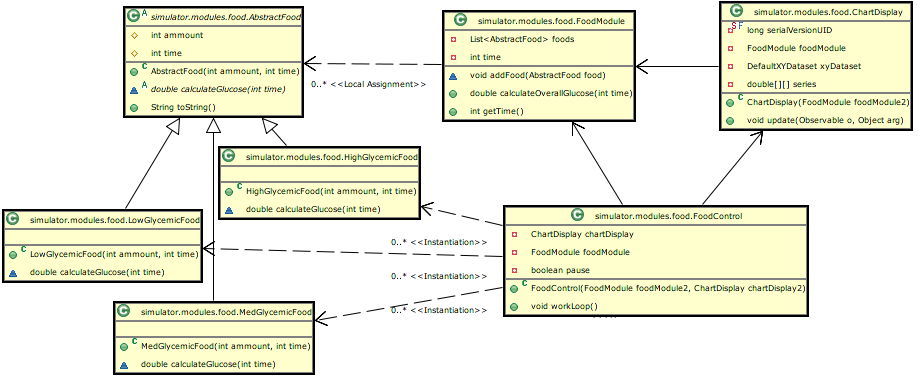
\includegraphics[width=\textwidth]{images/food_module_class_diagram2.png}
\caption{Food Module Class Diagram}
\label{fig:food_module_class_diagram}
\end{figure}

\subsubsection{Insulin}

\newpage
\subsection{Body Simulation}
For implementing the body simulation and putting all the behavioral modules
together while still providing large flexibility for further extensions and
changes the Model View Controller paradigm is used (see figure
\vref{fig:mvc_simplified}). 

\begin{figure}[htb]
\centering
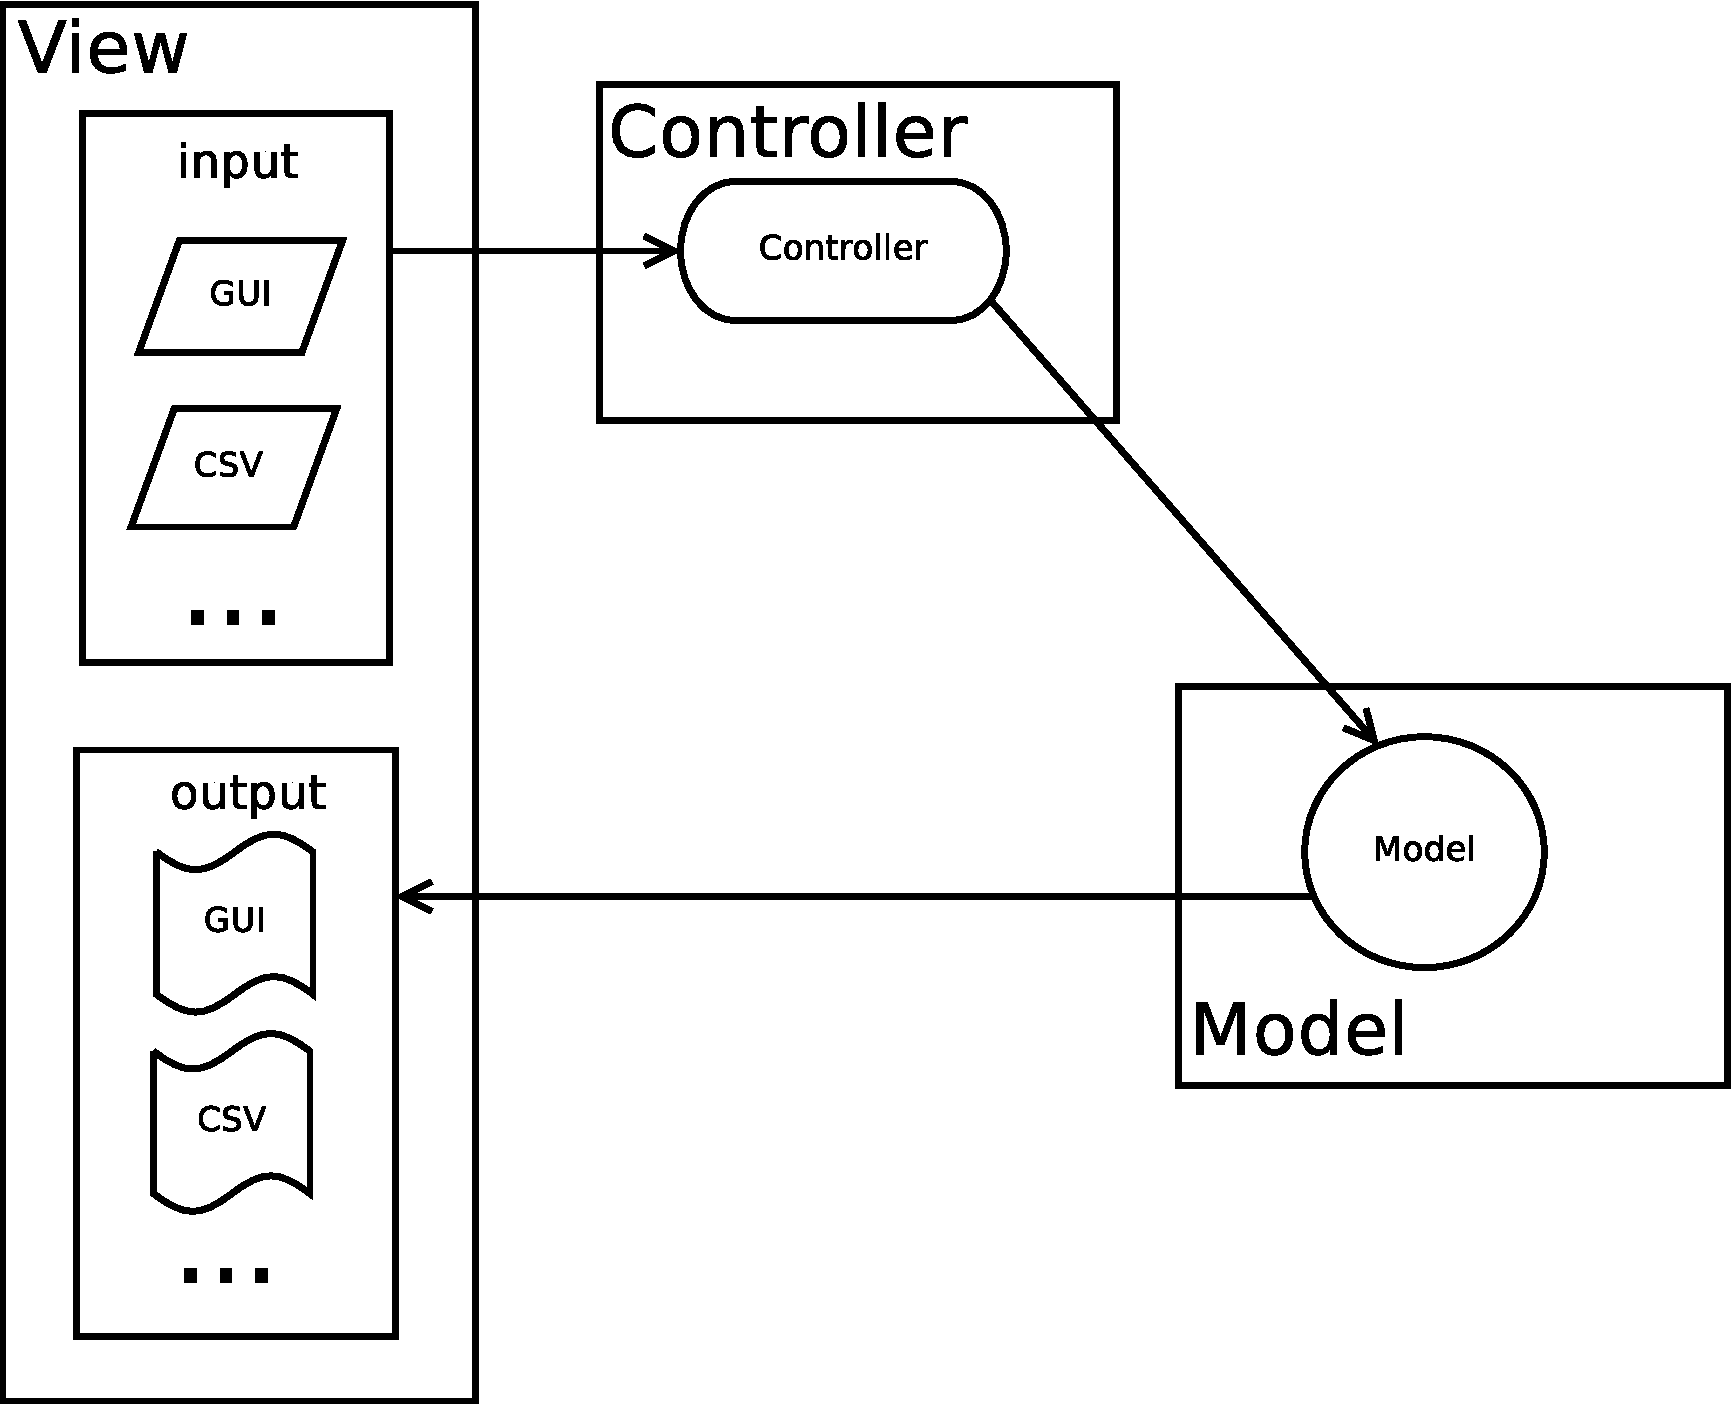
\includegraphics[scale=0.4]{images/mvc_simplified}
\caption{Simplified illustration of Model View Controller concept}
\label{fig:mvc_simplified}
\end{figure}

This should also allow an easy integration of the
components of the insulin pump which interact with the human body (i.e. sensor
and injection unit).
The resulting class design is as follows  (see figure
\vref{fig:body_simulation_class_diagram}): 

\begin{landscape}
\begin{figure}[htb]
\centering
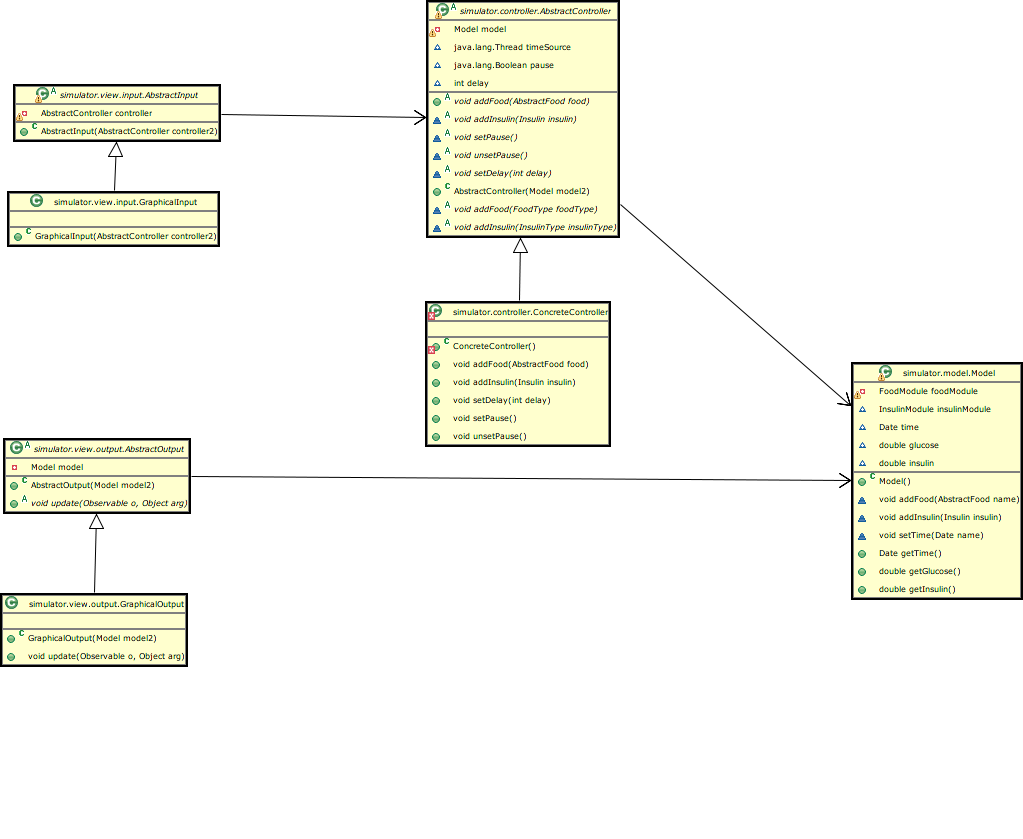
\includegraphics[width=\textwidth]{images/body_simulation_classdiagram.png}
\caption{Body Simulation Class Diagram}
\label{fig:body_simulation_class_diagram}
\end{figure}
\end{landscape}

\newpage
\subsection{Insulin Pump}
Thanks to the very open and felxible implementation of the Body Simulation
following the Model View Controller paradigm, the sensor and injector components
of the Insulin pump can be very easily integrated into the model.

\begin{figure}[htb]
\centering
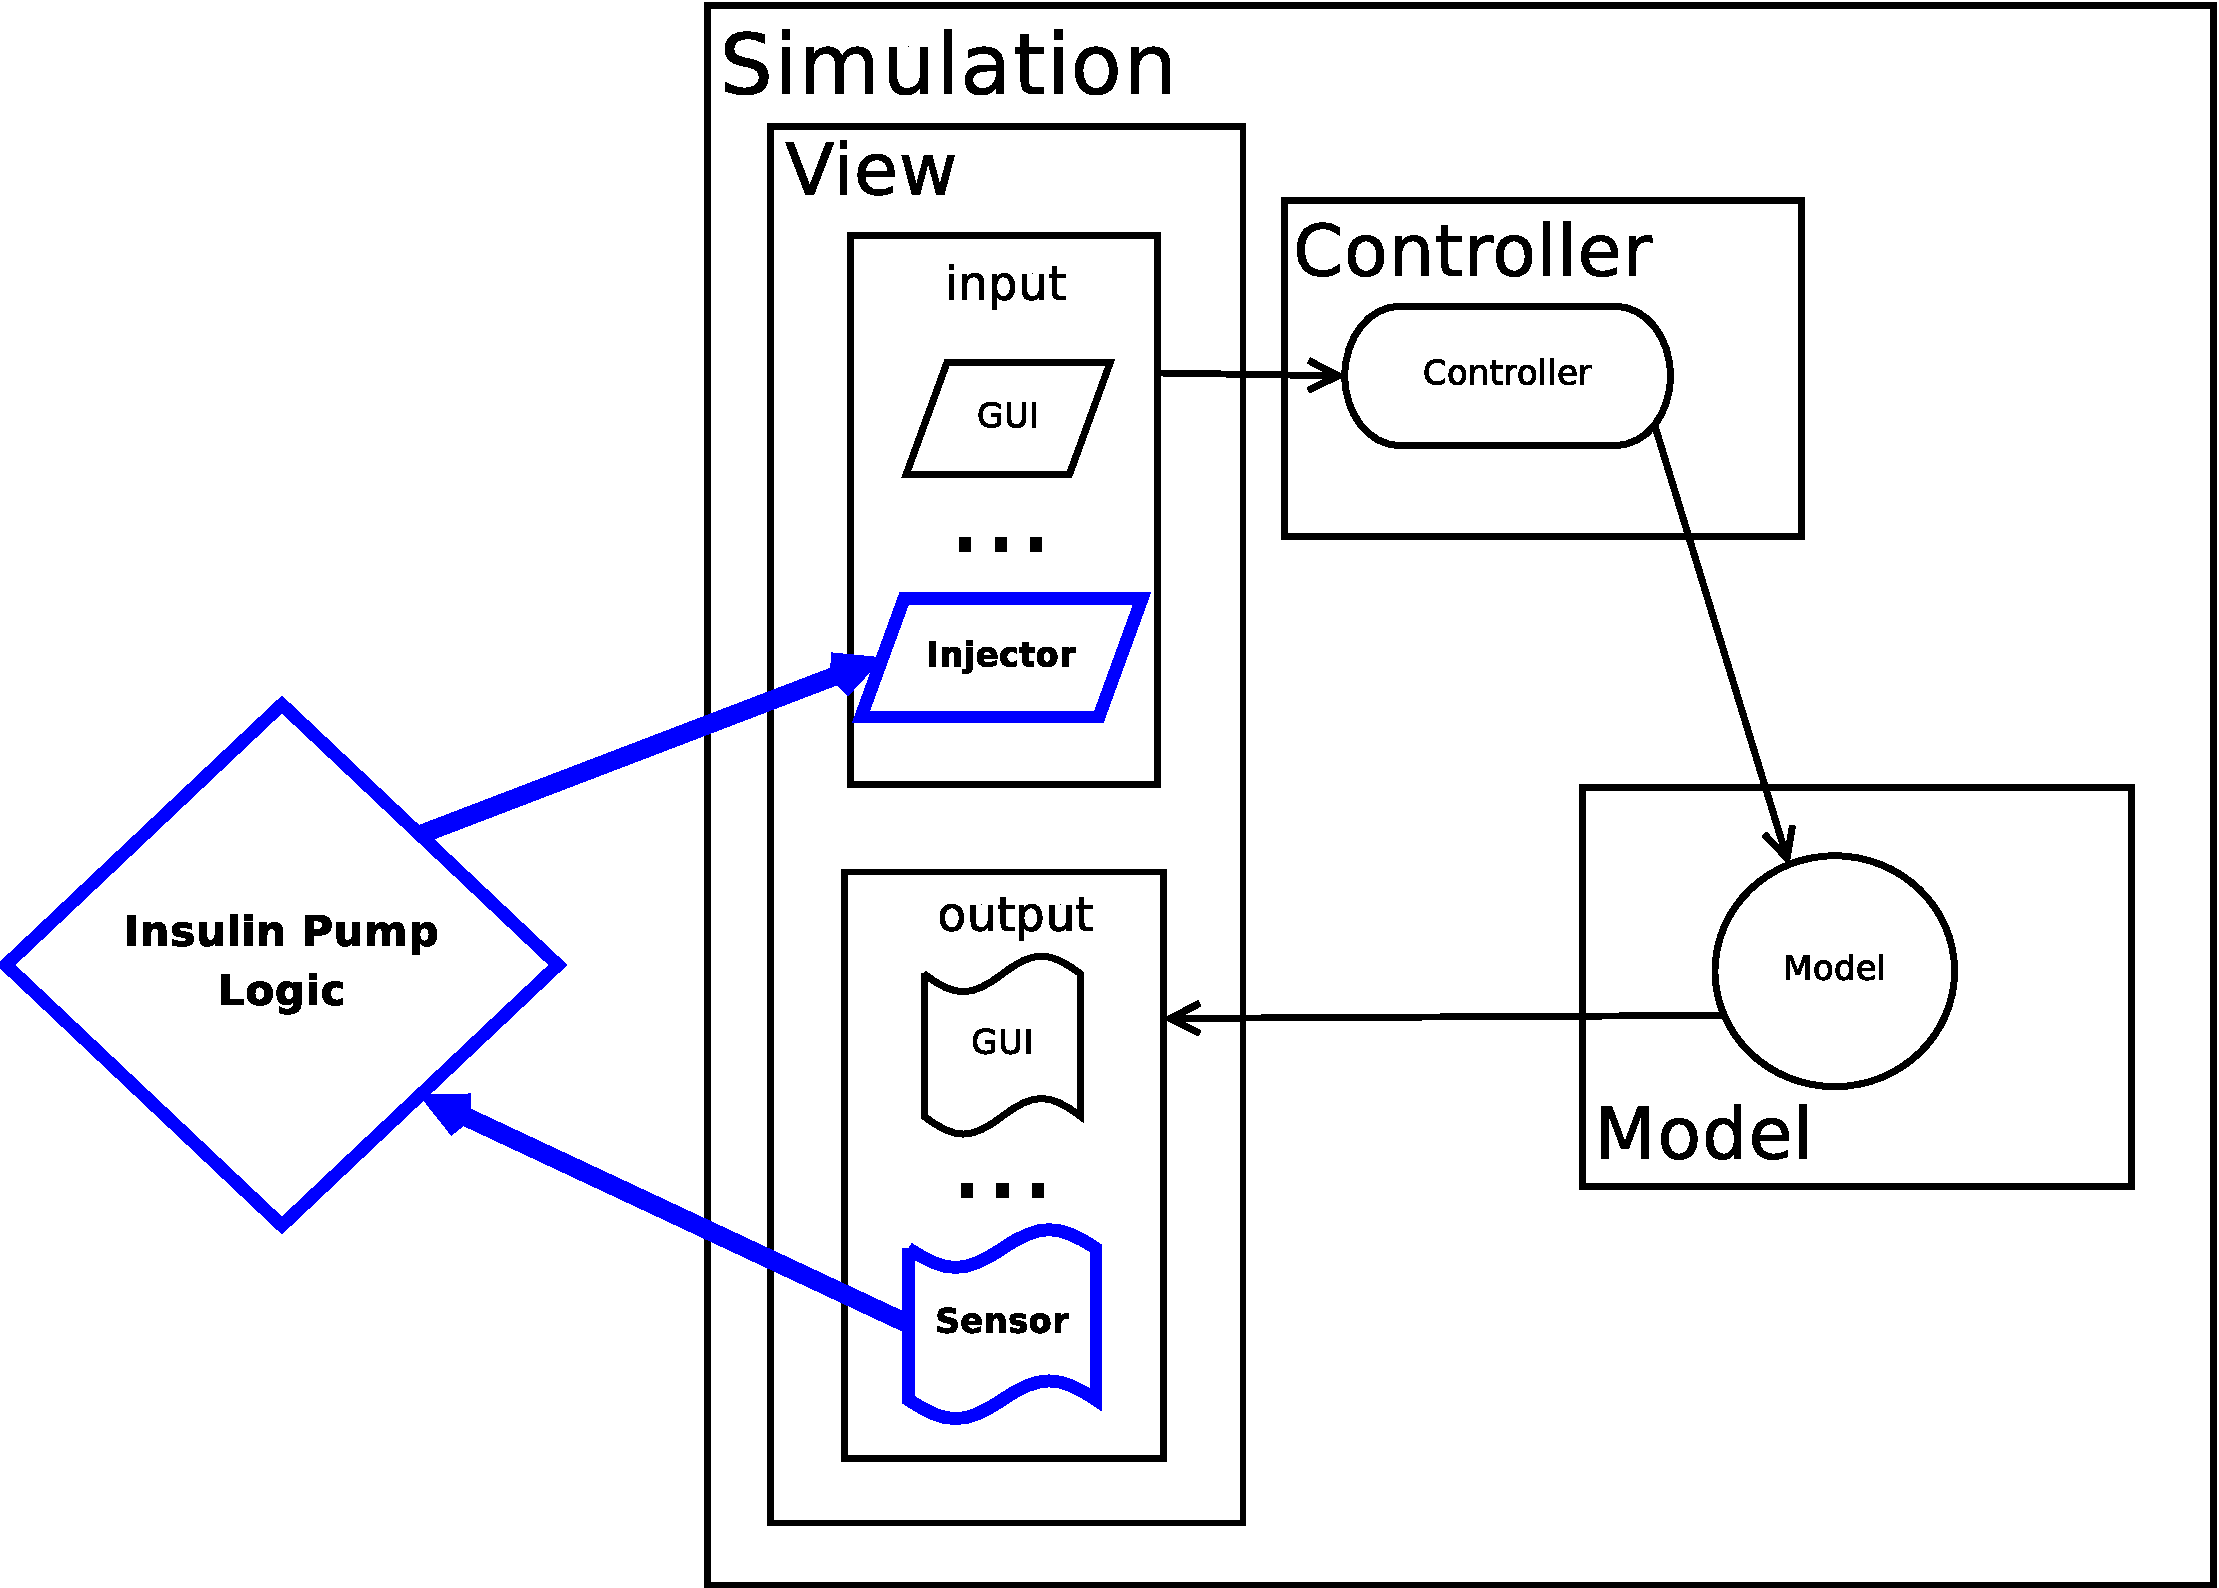
\includegraphics[scale=0.39]{images/mvc_insulin_pump}
\caption{Integration of the Insulin Pump into the Body Simulation}
\label{fig:mvc_insulin_pump}
\end{figure}
